\begin{figure} [htb!]
\begin{longtable}{|p{18cm}|}
\hline
\textbf{Brugsmønster: }Opret sag \\
\hline
\textbf{ID: }1 \\
\hline
\textbf{Primære aktører: }Sagsbehandler, afdelingsleder, administrativt personale\\
\hline
\textbf{Sekundære aktører: }CPR\\
\hline
\textbf{Kort beskrivelse: }En aktør kan oprette en sag, som gemmes i systemet. \\
\hline
\textbf{Prækonditioner: }Aktør skal være logget ind.\\
\hline
\textbf{Hovedhændelsesforløb: }\newline 
Starter når en borger henvender sig til kommunen \\
1. Aktør indtaster CPR nummer, borgers navn, begrundelse for henvendelse \\
2. Gemmer indtastet data.	
\\
\hline
\textbf{Postkonditioner: }sag oprettet\\
\hline
\textbf{Alternative hændelsesforløb: }\\
\hline
\end{longtable}
\caption{Brugsmønster for opret sag}
\label{tab:1}
\end{figure}

\begin{figure} [htb!]
\begin{longtable}{|p{18cm}|}
\hline
\textbf{Brugsmønster:} Behandle sag \\
\hline
\textbf{ID:} 2\\
\hline
\textbf{Primære aktører:} Sagsbehandler\\
\hline
\textbf{Sekundære aktører:} Handleplan modul\\
\hline
\textbf{Kort beskrivelse:}  Sagsbehandlerne starter behandling af en sag i forhold til indhentning af oplysninger, hvorefter sagen bliver vurderet. Efterfølgende kommer en sagsafgørelse og til sidst bestilles evt. ydelser. \\
\hline
\textbf{Prækonditioner:} Der skal være oprettet en sag. \\
\hline
\textbf{Hovedhændelsesforløb:}\\
Starter når sagsbehandler vælger “Behandle sag”.\\
1. Sagsbehandler udfylder en sagsåbningsformular.\\
2. hvis sagsåbningsformular ikke er udfyldt.\\
2.1 Alternativt hændelsesforløb Behandle sag : Manglende information\\
3. hvis sagsåbningsformular er udfyldt\\
3.1 Udredningsformularen udfyldes med dataer fra  sagsåbningsformular.\\
3.2 Der bliver sendt data til handleplan modulet ift. oprettelse af en handleplan. \\
3.3 Der vælges mellem alternativt forløb indhent oplysninger eller sagsafgørelse.\\
\\
\hline
\textbf{Postkonditioner: }none\\
\hline
\textbf{Alternative hændelsesforløb: }Indhente oplysninger fra eksterne kilder, Afgøre sagsbehandling, Manglende information\\
\hline
\end{longtable}
\label{tab:2}
\caption{Brugsmønster for behandle sag}
\end{figure}

\begin{figure} [htb!]
\begin{longtable}{|p{18cm}|}
\hline
\textbf{Alternativ hændelsesforløb:} Behandle sag: Indhente oplysninger fra eksterne kilder \\
\hline
\textbf{ID:} 2.1 \\
\hline
\textbf{Primære aktører:} Sagsbehandler\\
\hline
\textbf{Sekundære aktører:} Sundhedssystem \\
\hline
\textbf{Kort beskrivelse: }Indhenter oplysninger fra eksterne systemer\\
\hline
\textbf{Prækonditioner: }Der skal være en udredningsformularen der er påbegyndt\\
\hline
\textbf{Alternativhændelsesforløb:}\\
1. Indtastning af oplysninger i relevante felter fra eksterne kilder i udredningsformularen.\\
2. Formularen gemmes\\
3. Sagen lukkes\\
\\
\hline
\textbf{Postkonditioner:} Formularen opdateret \\
\hline
\end{longtable}
\caption{Alternativ hændelsesforløb for behandle sag}
\label{tab:2.1}
\end{figure}

\begin{figure} [htb!]
\begin{longtable}{|p{18cm}|}
\hline
\textbf{Alternativ hændelsesforløb:} Behandle sag : Afgøre sagsbehandling \\
\hline
\textbf{ID:} 2.2 \\
\hline
\textbf{Primære aktører:} Sagsbehandler\\
\hline
\textbf{Sekundære aktører:} Handleplan modul, Dagbog modul \\
\hline
\textbf{Kort beskrivelse: }Sagsbehandler registrerer afgørelse af pågældende sag og skriver et brev til borger omkring afgørelsen. Hvis sagen ikke er afvist, udfyldes en bestilling af social indsats.\\
\hline
\textbf{Prækonditioner: }Der er indhentet oplysninger fra eksterne kilder. 
\\
\hline
\textbf{Alternativhændelsesforløb:}\\
1. Hvis sagen ikke afvises.\\
1.1 Udfylder formularen for bestilling af social indsats\\
1.2 Systemet sender oplysninger til handleplan modulet ift. færdiggørelse af handleplanen.\\
1.3 Systemet sender oplysninger til dagbog modulet ift.  oprettelse af dagbog.\\
2. Der udfyldes et afgørelsesbrev. \\
3. Afgørelsesbrevet gemmes.\\
4. Sagen lukkes.
\\
\hline
\textbf{Postkonditioner:} Sagen er opdateret. Der skal være udfyldt et afgørelsesbrev.  \\
\hline
\end{longtable}
\caption{Alternativ hændelsesforløb for behandle sag}
\label{tab:2.2}
\end{figure}

\begin{figure} [htb!]
\begin{longtable}{|p{18cm}|}
\hline
\textbf{Alternativ hændelsesforløb:} Behandle sag : Manglende information\\
\hline
\textbf{ID:} 2.3 \\
\hline
\textbf{Primære aktører:} Sagsbehandler\\
\hline
\textbf{Sekundære aktører:} none \\
\hline
\textbf{Kort beskrivelse: }Bruges i tilfælde af at en sagsåbningsformular ikke er tilstrækkeligt udfyldt.
\\
\hline
\textbf{Prækonditioner: }Der skal være startet en sag, med delvist udfyldt formular. 
\\
\hline
\textbf{Alternativhændelsesforløb:}\\
1. Starter ved mangel på information i trin 2 i behandle sag.
2. Når formularen genoptages.
2.1 Åbnes formularen og manglende information udfyldes. 
3. Hvis formularen er udfyldt.
3.1 Gå til trin 3 i behandle sag.

\\
\hline
\textbf{Postkonditioner:} none\\
\hline
\end{longtable}
\caption{Alternativ hændelsesforløb for behandle sag}
\label{tab:2.3}
\end{figure}

\begin{figure} [htb!]
\begin{longtable}{|p{18cm}|}
\hline
\textbf{Brugsmønster: }Find sag \\
\hline
\textbf{ID: }3\\
\hline
\textbf{Primære aktører: }Sagsbehandler\\
\hline
\textbf{Sekundære aktører: }none\\
\hline
\textbf{Kort beskrivelse: }Skal kunne søge i sager og få en sag vist\\
\hline
\textbf{Prækonditioner: }Der skal være oprettet en eller flere sager\\
\hline
\textbf{Hovedhændelsesforløb: }\\
Starter når den primære aktør skal finde en sag.\\
1. Skal søge en sag på sagsnummer, CPR nummer, eller navn.\\
2. Vise en liste over de sager som blev fundet.\\
3. Hvis en sag bliver valgt.\\
3.1 Vis den valgte sag.\\
\hline
\textbf{Postkonditioner: }\\
\hline
\textbf{Alternative hændelsesforløb: }\\
\hline
\end{longtable}
\caption{Brugsmønster for find sag}
\label{tab:3}
\end{figure}

\begin{figure}[hbt!]
  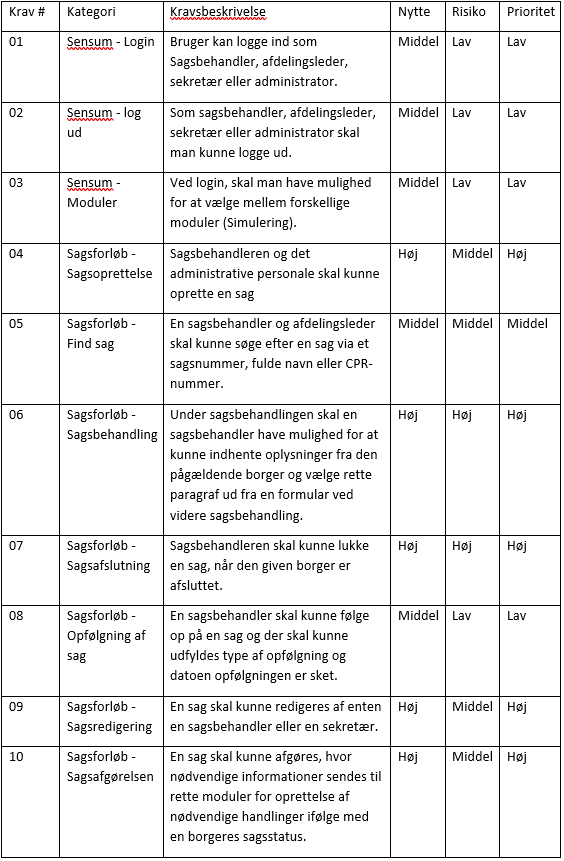
\includegraphics[scale = 0.9]{./PNG/krav/krav.PNG} 
  \caption{Funktionelle krav for projektet}
  \label{fig:krav}
\end{figure}

\begin{figure}[hbt!]
  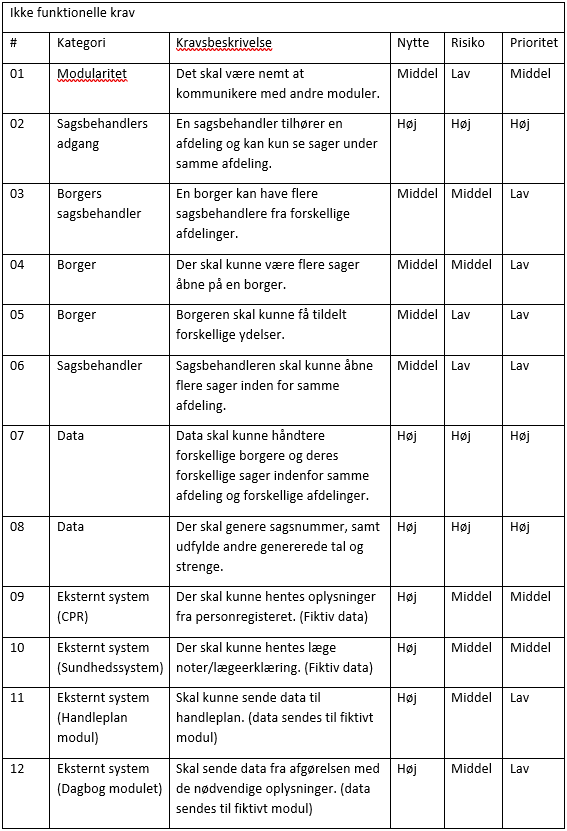
\includegraphics[scale = 0.9]{./PNG/krav/ikkeKrav.PNG} 
  \caption{ikke funktionelle krav for projektet  }
  \label{fig:ikkeKrav}
\end{figure}